% !TEX root = ../main.tex
% SECTION 3: KAPAZITÄT UND DIELEKTRIKA
% ============================================================

\StartChapter{Kapazität und Dielektrika}

\begin{runintext}
Formeln zu \ZSFkeyword*{Kapazitäten} und \ZSFkeyword*{Dielektrika}: Definition der Kapazität, typische Geometrien (Platte, Zylinder, Kugel), gespeicherte Energie und \ZSFkeyword*{Energiedichte}, \ZSFkeyword*{Reihen-} und \ZSFkeyword*{Parallelschaltungen} sowie Einfluss von Dielektrika. Nützlich bei Aufgaben zu \ZSFkeyword*{Kondensatoren}, Energiespeicherung, Schaltungen und Feldänderungen durch Materialeinbau.
\end{runintext}

\SubsectionBar[sec:capacitance]{Kapazität}
\ZSFindexsee{Farad}{Kapazität}
\begin{runintext}
Grundformeln für Spannung und \ZSFkeyword{Kapazität} von \ZSFkeyword[Kondensator]{Kondensatoren}; nützlich, wenn aus Ladung und Spannung die Kapazität oder umgekehrt gesucht ist.
\end{runintext}
\begin{defbox}[Kondensator]
Zwei \ZSFkeyword*{isolierte Leiter} mit gleich grosser, entgegengesetzter Ladung; speichert Ladung und Energie.
\end{defbox}
\begin{formulabox}
\[ U = \overbrace{\varphi_b - \varphi_a}^{\text{Potentialdiff.}} \quad \text{Spannung } [\si{V}] \]
\formulasep
\[ C = \frac{q}{U} \quad \text{Kapazität } [\si{F} = \si{C/V}] \]
\formulanote{Zweck: Spannung zwischen Leitern; Definition Kapazität (Ladung pro Spannung).}
\end{formulabox}
\begin{runintext}
\ZSFkeyword*{Einzelleiter}: $q$ Gesamtladung, $U$ gegen Unendlich. \ZSFkeyword{Kondensator}: $q$ Ladung auf einem Leiter, $U$ zwischen den Leitern.
\end{runintext}

\ZSFfig{graphics/kondensator_grafik.png}{Kondensator mit Spannungsquelle}{Ladung $q$ proportional zur Spannung $U$: $C=q/U$}

\SubsectionBar[sec:capacitor-energy]{Energie Kondensator}
\ZSFindex{Energie / elektrische Energie}
\ZSFindex{Energiedichte}
\begin{runintext}
Formeln für Energie und \ZSFkeyword[Energie/Energiedichte Kondensator]{Energiedichte} im Kondensatorfeld; nützlich bei Energiespeicher-Aufgaben und Feldstärkeabschätzungen.
\end{runintext}
\begin{formulabox}
\[ E_{\mathrm{el}} = \frac{1}{2}\,qU = \frac{q^2}{2C} = \frac{1}{2}\,CU^2 \]
\formulanote{Zweck: Im Kondensator gespeicherte Energie. \ZSFdanger{Achtung:} Beim Laden an konstanter Quelle geht 50\% der Energie als Wärme verloren!}
\formulasep
\[ w_{\mathrm{el}} = \frac{1}{2}\,\varepsilon_0 E^2 \quad \text{Energiedichte} \]
\[ E_{\mathrm{el}} = w_{\mathrm{el}}\,V \quad \text{(homogenes Feld)} \]
\formulanote{Zweck: Elektrische Energiedichte im Feld; Gesamtenergie bei homogenem Feld über Volumen $V = A \cdot d$ (Fläche $A$, Abstand $d$).}
\end{formulabox}

\SubsectionBar[sec:capacitor-geometries]{Platte, Zylinder, Kugel}
\ZSFindex{Plattenkondensator}
\ZSFindex{Zylinderkondensator}
\ZSFindex{Kugelkondensator}
\begin{runintext}
Spezielle Kapazitäten typischer Geometrien (\ZSFkeyword*{Platte}, \ZSFkeyword{Koaxkabel}, \ZSFkeyword*{Kugel}). \textbf{Herkunft}: Ladung $q$ ansetzen $\to$ Feld via Gauss \ZSFref{sec:gauss-law} $\to$ Spannung $U = \int_{+}^{-} \vec{E}\cdot\mathrm{d}\vec{s}$ \ZSFref{sec:potential-difference} $\to C = q/U$.
\end{runintext}

\begin{defbox}[Plattenkondensator (Fläche $A$, Abstand $d$)]
\begin{splitbox}[0.3]
    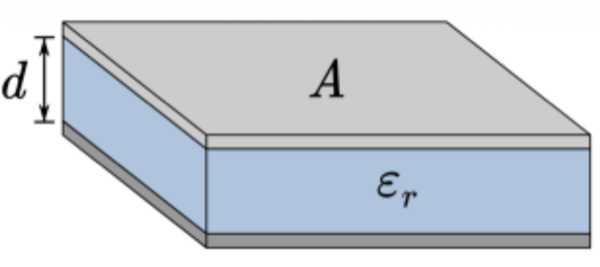
\includegraphics[width=\linewidth, keepaspectratio]{graphics/Elektrotechnik_Plattenkondensator_Dielektrikum_Modell.png}
    \tcblower
    \begin{formulabox}
        \textVorFormel{Elektrisches Feld (homogen):}
        $E = \frac{U}{d} = \frac{Q}{\varepsilon_0\,A} = \frac{\sigma}{\varepsilon_0}$\par
        \tcbline
        \textVorFormel{Kapazität:}
        $C = \frac{\varepsilon_0\,A}{d}$
    \end{formulabox}
\end{splitbox}
\tcbline
\ZSFdanger{Teilweises Dielektrikum:} Deckt es nicht den gesamten Plattenbereich:
\par\ZSFgapXS
\centering
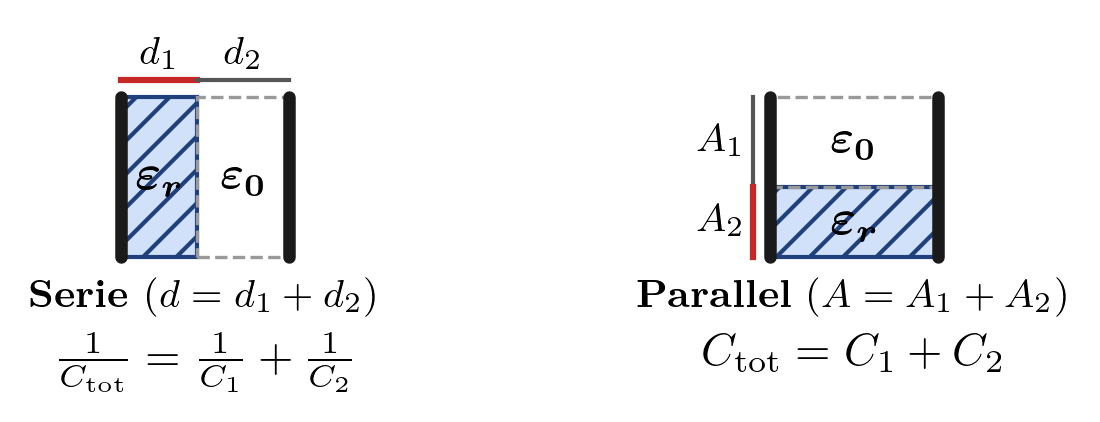
\includegraphics[width=\linewidth, keepaspectratio]{graphics/Plattenkondensator_Teilweises_Dielektrikum.png}
\end{defbox}

\begin{defbox}[Zylinderkondensator (Länge $\ell$, $r_2>r_1$)]
\begin{splitbox}[0.3]
    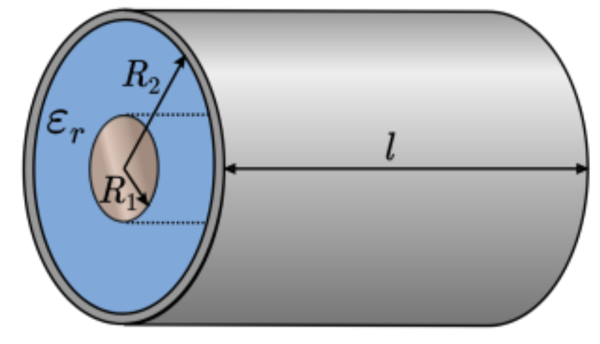
\includegraphics[width=\linewidth, keepaspectratio]{graphics/Physik_Koaxialleiter_Dielektrikum_Epsilon_r.png}
    \tcblower
    \begin{formulabox}
        \textVorFormel{Kapazität:}
        $C = \frac{2\pi\varepsilon_0\,\ell}{\ln(r_2/r_1)}$\par
        \tcbline
        \textVorFormel{Elektrisches Feld (radial):}
        $E(r) = \frac{U}{r\,\ln(r_2/r_1)}$
    \end{formulabox}
\end{splitbox}
\end{defbox}

\begin{defbox}[Kugelkondensator (konz.\ Sphären, $r_1<r_2$)]
\begin{splitbox}[0.3]
    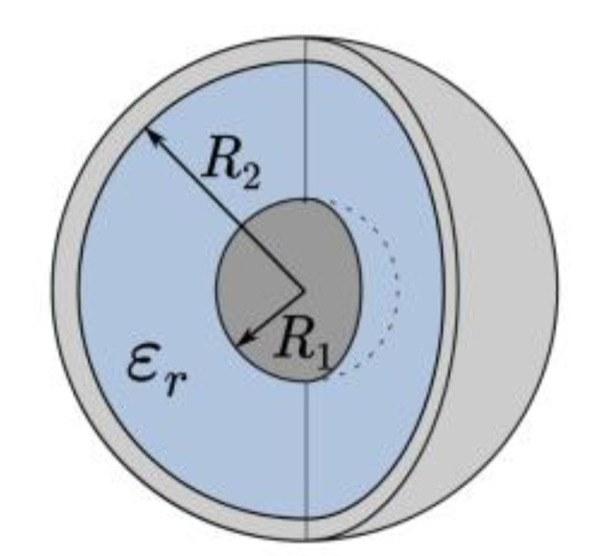
\includegraphics[width=\linewidth, keepaspectratio]{graphics/physik_concentric_spheres_dielectric_epsilon_r.png}
    \tcblower
    \begin{formulabox}
        \textVorFormel{Kapazität:}
        $C = 4\pi\varepsilon_0\,\frac{r_1\,r_2}{r_2 - r_1}$\par
        \tcbline
        \textVorFormel{Einzelkugel (Grenzfall $r_2\to\infty$):}
        $C = 4\pi\varepsilon_0\,r$
    \end{formulabox}
\end{splitbox}
\end{defbox}

\columnbreak
\SubsectionBar[sec:capacitors-series]{Reihenschaltung}
\ZSFindex{Reihenschaltung / Serienschaltung}
\begin{runintext}
Ersatzkapazität bei \ZSFkeyword[Reihenschaltung / Serienschaltung]{Serie}. Gleiche Ladung, Spannungen addieren sich (\ZSFkeyword{Maschenregel} $\sum U_k = 0$).
\end{runintext}
\begin{defbox}[Serienschaltung]
\begin{splitbox}[0.45]
    \centering
    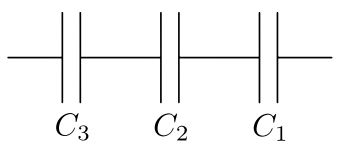
\includegraphics[width=\linewidth, keepaspectratio]{graphics/kondensatorserie.png}
    \tcblower
    \begin{formulabox}
        \[ \frac{1}{C_{\mathrm{tot}}} = \sum_k \frac{1}{C_k} \]
        \formulasep
        \[ U_{\mathrm{tot}} = U_1 + U_2 + U_3 + \cdots \]
        \[ U_k = \frac{C_{\mathrm{tot}}}{C_k} \cdot U_{\mathrm{tot}} \]
        \[ I = I_1 = I_2 = I_3 \]
        \[ Q = Q_1 = Q_2 = Q_3 \]
    \end{formulabox}
\end{splitbox}
\formulanote{Gleiche Ladung $Q$ auf allen Kondensatoren. Reihe: Trennt weniger Ladung, da sich Plattenabstände addieren.}
\end{defbox}

\SubsectionBar[sec:capacitors-parallel]{Parallelschaltung}
\begin{runintext}
Ersatzkapazität bei \ZSFkeyword[Parallelschaltung]{Parallel}. Gleicher Spannungsabfall, Ladungen addieren sich.
\end{runintext}
\begin{defbox}[Parallelschaltung]
\begin{splitbox}[0.45]
    \centering
    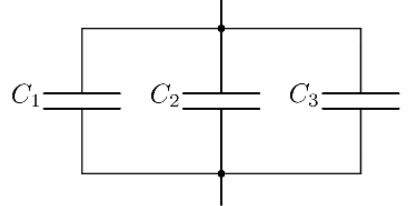
\includegraphics[width=\linewidth, keepaspectratio]{graphics/kondensatorparallel.png}
    \tcblower
    \begin{formulabox}
        \[ C_{\mathrm{tot}} = C_1 + C_2 + C_3 + \cdots \]
        \formulasep
        \[ U_k = U_{\mathrm{tot}} \quad (\forall k) \]
        \[ I_{\mathrm{tot}} = I_1 + I_2 + I_3 \]
        \[ Q_{\mathrm{tot}} = Q_1 + Q_2 + Q_3 + \cdots \]
    \end{formulabox}
\end{splitbox}
\formulanote{Gleiche Spannung $U$ an allen Kondensatoren. Parallel: Trennt mehr Ladung, da sich Plattenflächen addieren.}
\end{defbox}

\SubsectionBar[sec:dielectrics]{Dielektrika}
\ZSFindex[Vakuumpermittivitat/-permeabilitat]{Vakuumpermittivität/-permeabilität}
\ZSFindex{Relative Permittivität}
\ZSFindexsee{Permittivität}{Relative Permittivität}
\begin{runintext}
Formeln, wie isolierende Materialien (\ZSFkeyword{Dielektrika}) das Feld und die Kapazität verändern; nützlich beim Einbau von Medien zwischen Platten.
\end{runintext}
\begin{formulabox}
\[ C = \varepsilon_{\mathrm{rel}} C_0 \]
\[ \varepsilon = \varepsilon_{\mathrm{rel}}\varepsilon_0 \]
\formulasep
\[ \vec{D} = \varepsilon_{\mathrm{rel}}\varepsilon_0 \vec{E} \quad \text{Elektrische Verschiebungsdichte} \]
\formulanote{Zweck: Kapazität $C$ mit Dielektrikum steigt gegenüber Vakuumkapazität $C_0$ um $\varepsilon_{\mathrm{rel}}$ (rel. Dielektrizitätskonstante).}
\end{formulabox}
\begin{propertylist}[Verhalten beim Einschub eines Dielektrikums]
  \ZSFFact{Mit Spannungsquelle}{Spannung $U$ bleibt konstant. $C$ steigt proportional zu $\varepsilon_{\mathrm{rel}}$. Damit fliesst Ladung nach ($q$ steigt). Das \ZSFkeyword*{elektrische Feld} $\vec{E}$ bleibt konstant ($E = U/d$).}
  \ZSFFact{Ohne Spannungsquelle}{Ladung $q$ bleibt konstant (kann nicht ab- oder zufliessen). $C$ steigt. Spannung $U$ sinkt ($U=q/C$), und das \ZSFkeyword*{elektrische Feld} sinkt proportional ($E = E_0 / \varepsilon_{\mathrm{rel}}$).}
\end{propertylist}
\begin{runintext}
Mikroskopisch: \ZSFkeyword[Dipol]{Dipole} richten sich aus, erzeugen Gegenfeld. Anwendung: höhere Kapazität, \ZSFkeyword*{Durchschlagfestigkeit}, mechanische Trennung.
\end{runintext}

\ZSFfig{graphics/Kondensator_mit_und_ohne_Dielektrikum.jpg}{Mit/ohne Dielektrikum}{Polarisierte Dipole schwächen $\vec{E}$ im Inneren}

% ============================================================
